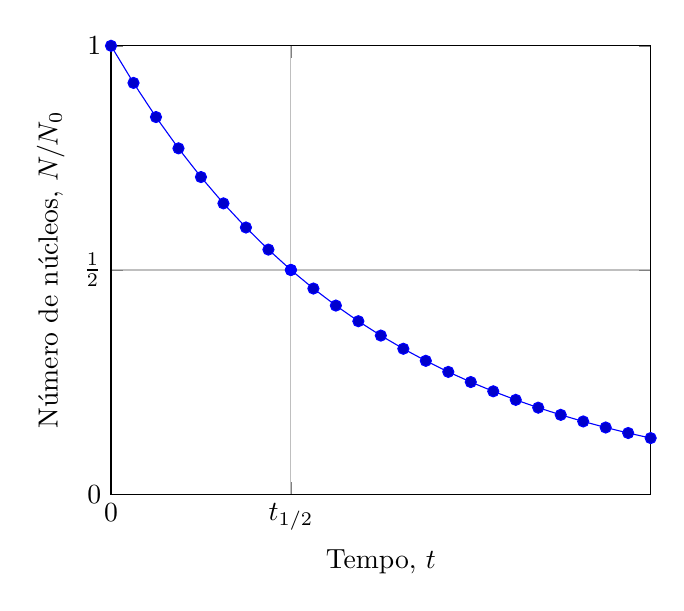
\begin{tikzpicture}
    \begin{axis}
        [
            grid = major,
            xlabel = {Tempo, $t$},
            ylabel = {Número de núcleos, $N/N_0$},
            xmin = 0, xmax = 3,
            ymin = 0, ymax = 1,
            domain = 0:3,
            ytick = {0, 0.5, 1},
            yticklabels = {0, $\frac{1}{2}$, 1},
            xtick = {0, 1},
            xticklabels = {0, $t_{1/2}$},
        ]
    \addplot 
        { 2^(-x) };
    \addplot[mark=*, color=blue] coordinates
        { (1,0.5) };

    \end{axis}
\end{tikzpicture}